\documentclass[main.tex]{subfiles}

\begin{document}

\providecommand{\Par}{\operatorname{Parent}}
\newcommand{\LA}{\operatorname{LA}}
\newcommand{\Dep}{\operatorname{D}}
\newcommand{\LCA}{\operatorname{LCA}}

\newcommand{\NZ}{\operatorname{NZ}}
\newcommand{\CSB}{\textit{CSB}}
\renewcommand{\V}{\operatorname{V}}
\newcommand{\R}{\operatorname{R}}
\newcommand{\J}{\operatorname{J}}


\chapter{Ancestors with skew-binary representation} \label{cap:skew}

In this chapter, we present another solution for the Level Ancestor problem. This solution, despite being a little more complicated, requires preprocessing that consumes constant time and space per added node. This solution was initially given by Myers~\cite{Myers83}. In the end of the chapter, we also present the solution to the Lowest Common Ancestor problem using the same technique.

As we'll deal with numerical representations extensively, in this chapter we'll also use chain notation, in which~$21^5$ represents the chain~$211111$ and not the number~$4084101$.

\section{Definition and properties}

A \deff{skew-binary} number of length~$n$ is the chain~${a = a_n a_{n-1} \cdots a_1}$ such that~${a_i \in \{0, 1, 2\}}$ and~$a_n \neq 0$. We denote the length of~$a$ by~$|a| \coloneqq n$. The~\deff{value} of such number is~${\V(a) \coloneqq \sum\limits_{i = 1}^n{a_i (2^i - 1)}}$. Notice that multiple chains might have the same value, for example, both~21 and~100 both have value~7.

For all~$a$ such that~$\V(a) \neq 0$, define~$\NZ(a) \coloneqq \min\{i \in [n] : a_i \neq 0\}$, that is, the position of least significant non-zero digit of~$a$. We say a skew-binary number is~\deff{canonical} if all its digits are~0 or~1 except for, possibly, its least significant non-zero digit. More formally,~${a_i = 2}$ implies that~${i = \NZ(a)}$. Let~$\CSB$ be the set of all canonical skew-binary numbers.


This equality will be useful on the proof of the following lemmas:

\begin{equation} \tag{A} \label{eq:sum2}
	\sum\limits_{i = \ell}^r{2^i} = 2^{r+1} - 2^{\ell}.
\end{equation}

\begin{lemma} \label{lem:csbdig}
    If~$a \in \CSB$ and~$|a| = n$, then~$2^n - 1 \leq \V(a) \leq 2^{n+1}-2$.
\end{lemma}
\begin{proof}
    Consider the number~$b = 10^{n-1}$. By definition,~$a_n \geq 1 = b_n$ and~$a_i \geq 0 = b_i$ for~$i \in [n - 1]$, thus~$\V(a) \geq \V(b) = 2^n - 1$.

    For the other side of the inequality, consider
	\begin{align*}
	\V(a) = \sum\limits_{i = \NZ(a)}^n{a_i (2^i - 1)} &\stackrel{\text{(1)}}{\leq} \left(\sum\limits_{i = \NZ(a) + 1}^n (2^i - 1)\right) + 2 (2^{\NZ(a)} - 1) \\
	&\stackrel{\text{(2)}}{=} 2^{n+1} - 2^{\NZ(a)+1} - (n - \NZ(a)) + 2^{\NZ(a) + 1} - 2 \\
	&\stackrel{\text{(3)}}{\leq} 2^{n+1} - 2,
	\end{align*}
	where~(1) follows from~$a \in \CSB$,~(2) follows from~\eqref{eq:sum2} and~(3) follows from~$\NZ(a) \leq n$.
\end{proof}

The lemma shows that the smallest and the largest~$n$-digit number in CSB are~$10^{n-1}$ e~$20^{n-1}$, respectively, and also that any representation of~$x$ in CSB uses~$\floor{\lg(x + 1)}$ digits.


\begin{theorem} \label{thm:csbbij}
    Each positive integer has an unique representation in CSB. Alternatively,~${\V: \CSB \rightarrow \mathbb{N}}$ is a bijection.
\end{theorem}
\begin{proof}
    Let's first prove that~$\V$ is an injection, that is, if~${a \neq b}$ then~${\V(a) \neq \V(b)}$. Suppose, without loss of generality, that~$|a| \geq |b|$. If~$|a| > |b|$ then, by~Lemma~\ref{lem:csbdig},
	$$ \V(a) \geq 2^{|a|} - 1 > 2^{|a|} - 2 \geq 2^{|b| + 1} - 2 \geq \V(b). $$
    If~$|a| = |b|$, let~${i^\star \coloneqq \max\{i \in [n] : a_i \neq b_i\}}$. Suppose, without loss of generality, that ~${a_{i^\star} > b_{i^\star}}$. Write~${a = \alpha a_{i^\star} \beta}$ and~${b = \alpha b_{i^\star} \gamma}$. Then
	$$ \V(a) - \V(b) \stackrel{\text{(1)}}{\geq} (2^{i^\star} - 1) + \V(\beta) - \V(\gamma) \stackrel{\text{(2)}}{\geq} (2^{i^\star} - 1) - (2^{i^\star} - 2) = 1, $$
	where~(1) follows from~$a_{i^\star} \geq b_{i^\star} + 1$,~(2) follows from~$\V(\beta) \geq 0$ and using Lemma~\ref{lem:csbdig} on~$\gamma$. This proves that~$\V(a) \neq \V(b)$, thus~$\V$ is an injection.

    To prove that~$\V$ is a surjection we need to prove that, for all~$x \in \mathbb{N}$, there exists~${a \in \CSB}$ such that~${\V(a) = x}$. By induction on~$n$, let's prove that, for all~${x \leq 2^{n+1} - 2}$, there exists~${a \in \CSB}$ such that~${\V(a) = x}$. If~$n = 0$, then~$a = 0$ is such that~$\V(a) = 0$. Suppose~$n \geq 1$ and every~${x \leq 2^n - 2}$ has an unique representation in~$\CSB$. Let~${2^n - 1 \leq y \leq 2^{n+1} - 2}$. If~$y = 2^{n+1} - 2$, we know that~${a = 20^{n-1} \in \CSB}$ and~$\V(a) = y$. Otherwise,
	$$y - (2^n - 1) < 2^{n+1} - 2 - (2^n - 1) = 2^n - 1.$$
    Therefore, there exists~$a \in \CSB$ such that~${\V(a) = y - (2^n - 1)}$, but then~$b = 1a \in \CSB$ and~$\V(b) = y$.
\end{proof}

Since each positive integer has an unique representation in~CSB, we can define a function~${\R: \mathbb{N} \rightarrow \CSB}$ such that~$\V(\R(x)) = x$ for all~$x \in \mathbb{N}$, that is,~$\R(x)$ is the canonical skew-binary representation of~$x$.


\begin{lemma} \label{lem:csbsub}
    Let~$a \in \CSB$ such that~$\V(a) > 0$. If~$\NZ(a) = 1$ then~$\V(a_n \cdots a_2 (a_1-1)) = \V(a) - 1$, otherwise~${\V(a_n \cdots a_{\NZ(a)+1} (a_{\NZ(a)} - 1) 2 0^{\NZ(a) - 2}) = \V(a) - 1}$.
\end{lemma}
\begin{proof}
    When~$\NZ(a) = 1$, it follows that~$a_1 \neq 0$, thus~${b \coloneqq a_n \cdots a_2 (a_1-1) \in \CSB}$. Furthermore,~${\V(a) - \V(b) = a_1 - b_1 = 1}$.

    When~$\NZ(a) > 1$, since the only digit in~$a$ that may be 2 is the~$\NZ(a)$-th one, we have that~${b \coloneqq a_n \cdots a_{\NZ(a)+1} (a_{\NZ(a)} - 1) 2 0^{\NZ(a) - 2} \in \CSB}$. Furthermore,
	$$ \V(a) - \V(b) = (a_{\NZ(a)} - b_{\NZ(a)}) (2^{\NZ(a)} - 1) - 2 (2^{\NZ(a) - 1} - 1) = 2^{\NZ(a)} - 1 - (2^{\NZ(a)} - 2) = 1. $$
\end{proof}

The lemma shows that subtracting by~1 in the value of a canonical skew-binary number consists in decreasing its least significant non-zero digit by one and, if it exists, increase to two the digit to the right of it.

\section{Jump pointers}

In the Level Ancestor problem, to evaluate~$\LA(k, u)$, we have a node~$u$ of depth~$\Dep(u)$ and want to determine its ancestor~$v$ of depth~${\Dep(v) = \Dep(u) - k}$. In the solution presented in Subsection~\ref{subsec:pot2}, each node had a pointer to its $2^x$-th ancestor, for all~${x \in \floor{\lg\Dep(u)}}$, and the node~$v$ was reached from~$u$ by skipping the distinct powers of two from the decomposition of~$k$.

This problem can be interpreted in another way. We have a number~$x$ and want to transform it into~$y \leq x$, at each step decreasing the value of~$x$. With this interpretation, on the solution in Subsection~\ref{subsec:pot2}, which attempts to transform~$\Dep(u)$ into~$\Dep(v)$, from each number we could subtract any power of two. Note that decreasing the value of a number by~$z$ is equivalent to choosing the~$z$-th ancestor of a node in a tree.

Let's consider an alternative solution to this problem, in which starting from a positive number~$x$ we can jump to the numbers~$x-1$ or~$\J(x)$, where~${\J(x) \coloneqq x - (2^{\NZ(\R(x))} - 1)}$, that is, if we consider~$\R(x)$, the canonical skew-binary representation of~$x$,~$\J(x)$ consists of decreasing by one the least significant non-zero digit of~$\R(x)$. For example, if~$x = 13$, then~${\R(x) = 120}$ and~${\J(x) = \V(110) = 10}$. The Figure~\ref{fig:ex_rj} displays the values of~$\R$ and~$\J$ for small values.

\begin{figure}[tbh]
\centering
\begin{tikzpicture}
\begin{tabular}{|c||c|c|}
\hline
$x$ & $\R(x)$ & $\J(x)$ \\ \hline
$0$ & $0$ & $0$ \\
$1$ & $1$ & $0$ \\
$2$ & $2$ & $1$ \\
$3$ & $10$ & $1$ \\
$4$ & $11$ & $3$ \\
$5$ & $12$ & $4$ \\
$6$ & $20$ & $3$ \\
$7$ & $100$ & $0$ \\
$8$ & $101$ & $7$ \\
$9$ & $102$ & $8$ \\
$10$ & $110$ & $7$ \\
$11$ & $111$ & $10$ \\
$12$ & $112$ & $11$ \\
$13$ & $120$ & $10$ \\
$14$ & $200$ & $7$ \\
$15$ & $1000$ & $0$ \\
\hline
\end{tabular}

\begin{scope}[-latex', xshift=0.05cm, yshift=3.5cm, y=0.48cm, out=30, in=-30]
\newcommand{\dedges}[2]{\path (0, -#1) edge[out=20, in=-20] (0, -#2); }
\newcommand{\dedge}[2]{\path (0, -#1) edge[shorten >=0.175cm] (0, -#2); }
\newcommand{\dedgel}[2]{\path (0, -#1) edge[shorten >=0.35cm] (0, -#2); }
\dedges{1}{0}
\dedges{2}{1}
\dedge{3}{1}
\dedges{4}{3}
\dedges{5}{4}
\dedge{6}{3}
\path (0, -7) edge[shorten >=0.175cm] (0, 0);
%\dedgel{7}{0}
\dedges{8}{7}
\dedges{9}{8}
\dedge{10}{7}
\dedges{11}{10}
\dedges{12}{11}
\dedge{13}{10}
\dedgel{14}{7}
\path (0, -15) edge[shorten >=0.38cm] (0, 0);
%\dedge{15}{0}
\path (1, 0) rectangle (0, 1);
\end{scope}
\end{tikzpicture}
\caption{Values of functions~$\R$ and~$\J$ for small values. \label{fig:ex_rj}}
\end{figure}

Consider the following algorithm, which transforms~$x$ in~$y$ (initially~$x > y$):
\begin{algorithm}[h]
\caption{Transforming~$x$ in~$y$ using~$x-1$ and~$\J(x)$. \label{lst:xysub}}
\begin{algorithmic}[1]
	\While{$x \neq y$}
		\If{$\J(x) \geq y$}
			\State $x = \J(x)$
		\Else
			\State $x = x - 1$
		\EndIf
	\EndWhile
\end{algorithmic}
\end{algorithm}

The algorithm is greedy in the sense that it always chooses to use~$\J$ when possible (e~${J(x) \leq x - 1}$). The correctness of the algorithm is clear, since it is always possible to achieve~$y$ using only~$x-1$, and~$x$ never becomes smaller than~$y$.

\begin{theorem} \label{thm:xysub}
    The algorithm in Code listing~\ref{lst:xysub} completes in~$\Oh(\lg x)$ iterations of the~\keyword{while}.
\end{theorem}
\begin{proof}

	Let~$a \coloneqq \R(x)$,~$b \coloneqq \R(y)$ and~$n \coloneqq |a|$. If~$|a| > |b|$, increase~$b$ by adding 0s to the left. Let~${i^\star = \max{i \in [n] : a_i \neq b_i^\}}}$, and write~${a = \alpha a_{i^\star} \beta}$ and~${b = \alpha b_{i^\star} \gamma}$. By the Lema~\ref{lem:csbdig}, we have that~$a_{i^\star} > b_{i^\star}$ and that~${\V(c) > \V(b)}$, where~${c \coloneqq b_n \cdots b_{i^\star + 1} (b_{i^\star} + 1) 0^{i^\star - 1}}$. Note that~$c_i \leq a_i$ for all~${i \in [n]}$, and we have that~${\NZ(a) \leq i^\star}$. If~${\NZ(a) < i^\star}$ it holds that~$a_{\NZ(a)} > 0 = c_{\NZ(a)}$, and if~$\NZ(a) = i^\star$ it holds that~${a_{\NZ(a)} = a_{i^\star} \geq b_{i^\star} + 1 = c_{i^\star}}$. Therefore~$a_{\NZ(a)} \geq c_{\NZ(a)}$, with equality only if~$a = c$. Thus if~$a \neq c$ we can decrease~$a_{\NZ(a)}$ by one, i.e.~$\J(\V(a)) \geq \V(c)$. We can repeat this argument until~$a = c$, i.e.~$x = \V(c)$. This part performs at most~${\sum\limits_{i = 1}^{i^\star}{a_i} \leq i^\star + 1}$ iterations, since each digit is at most~1, except for one of these, which can be~2.

	Let's prove that if~${a = b_n \cdots b_{i+1} (b_i + 1) 0^{i-1}}$ for some~$i \in [n]$, with~${x = \V(a)}$ and~${y = \V(b)}$, then the algorithm will complete in at most~$2i$ iterations. With that proven, starting from where we left off above, that is, from~${c = b_n \cdots b_{i^\star + 1} (b_{i^\star} + 1) 0^{i^\star - 1}}$, the algorithm performs at most~$2i^\star$ additional iterations. Thus the algorithm performs at most~${(i^\star + 1) + 2i^\star = 3i^\star + 1 \leq 3n+1 = \Oh(\lg x)}$ iterations in total, and the complexity will be proved.

	The proof will be by induction on~$i$. If~$i = 1$ then~${\J(x) = x - 1 = y}$ and the algorithm ends in one iteration.
	Suppose that~$i > 1$ and the hypothesis holds for values smaller than~$i$. If~${\NZ(b) \geq i}$, then~$b$ has a suffix of at least~$i - 1$ values 0. That is~${a = b_n \cdots b_{i + 1} (b_{i} + 1) b_{i - 1} \cdots b_1}$, and thus if we decrease~1 from~$a_{i}$ we have~$b$, that is,~${\J(\V(a)) = \V(b)}$, and the algorithm ends in one iteration.
	Otherwise,~${J(\V(a)) < \V(b)}$, and so~$x = x - 1$ is executed. By the Lemma~\ref{lem:csbsub},~${\R(x - 1) = b_n \cdots b_i 2 0^{i-2}}$, and it is clear that~${\V(20^{i-2}) \geq \V(b_{i-1} \cdots b_1)}$. Consider the value of~$b_{i-1}$:
	\begin{itemize}
		\item if~$b_{i-1} = 2$, then~$x - 1 = y$ and the algorithm terminates, totalling one iteration;
		\item if~$b_{i-1} = 1$, then we can apply the induction hypothesis (for~$x - 1$ and~$i - 1$) and have that the algorithm terminates in at most~$2(i - 1) + 1 < 2i$ iterations;
		\item if~$b_{i-1} = 0$, then~$\J(x - 1) > y$ and~$\R(\J(x - 1)) = b_n \cdots b_i 1 0^{i-2}$, so we can apply the induction hypothesis (for~$\J(x-1)$ and~$i-1$) and we have that the algorithm terminates in at most~$2(i-1) + 2 = 2i$ iterations.
	\end{itemize}
\end{proof}

Figure~\ref{fig:exxysub} shows an example of applying the algorithm in Code listing~\ref{lst:xysub}. The transformation from~$x = 59$ to~$x = 46$ corresponds to the first part of the proof of Theorem~\ref{thm:xysub}. The remainder corresponds to the second part.

\begin{figure}[H]
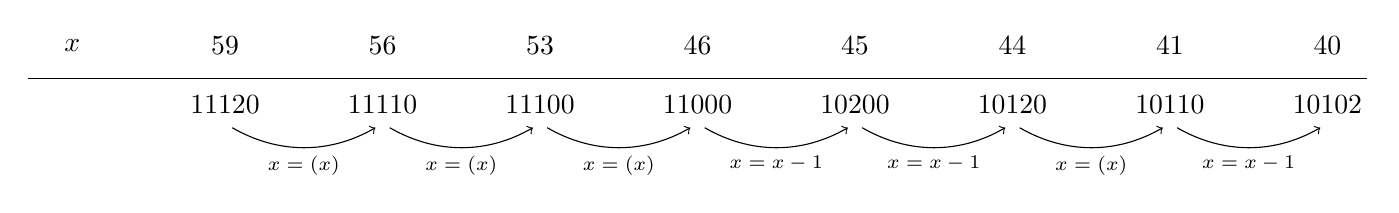
\begin{tikzpicture}
	%\draw (0, 1/10) node{x\ \ \ \ CSB\ \ };
	\draw (0, 3/4) node{\ \ $x$\ \ };
	\draw (0, 0) node{\ $\CSB$\ };
	%\draw (0, 0) grid (20, 10);
	\draw (-.5, 1/3) -- (16.5, 1/3);
	\foreach \i/\x/\csb in {1/59/11120, 2/56/11110, 3/53/11100, 4/46/11000, 5/45/10200, 6/44/10120, 7/41/10110, 8/40/10102}
	{
		\draw (\i+\i, 3/4) node{\ \x\ \ };
		\draw (\i+\i, 0) node(c\i){\csb};
	}
	\foreach \i/\j in {1/2, 2/3, 3/4, 6/7}
	{
		\draw (c\i.south) edge[bend right,->, shorten >=3pt, shorten <=3pt] node[below]{\scriptsize $x = \J(x)$} (c\j.south);
	}
	\foreach \i/\j in {4/5, 5/6, 7/8}
	{
		\draw (c\i.south) edge[bend right,->, shorten >=3pt, shorten <=3pt] node[below]{\scriptsize $x = x - 1$} (c\j.south);
	}
\end{tikzpicture}
\caption{Algorithm in Code listing~\ref{lst:xysub} applied on~$x = 59$ and~$y = 40$.} \label{fig:exxysub}
\end{figure}

\newcommand{\jmp}{\mathit{jump}}

Therefore, it is possible to use the same idea to solve the Level Ancestor problem. Suppose that every vertex~$u$ has a field~$u.\jmp$ that stores its ancestor with depth~$\J(\Dep(u))$. Then, analogously to the algorithm in Code~\ref{lst:xysub}, we can solve the Level Ancestor problem as in Code~\ref{lst:laskew}. The correctness is clear, and the time consumption~$\Oh(\lg\Dep(u))$ follows directly from Theorem~\ref{thm:xysub}.

\begin{algorithm}
\caption{Level Ancestor using the skew-binary representation.} \label{lst:laskew}
\begin{algorithmic}[1]
	\Function{LevelAncestor}{$k, u$}
		\State $y = \Dep(u) - k$
		\While{$\Dep(u) \neq y$}
			\If{$\Dep(u.\jmp) \geq y$}
				\State $u = u.\jmp$
			\Else
				\State $u = \Par(u)$
			\EndIf
		\EndWhile
		\State \Return $u$
	\EndFunction
\end{algorithmic}
\end{algorithm}

\section{Computing jump pointers}

The previous section presented a solution to the Level Ancestor problem in logarithmic time, but in it we assumed that each node~$u$ had a field~$u.\jmp$ with its~\mbox{$J(\Dep(u))$-th} ancestor. In this section, we will detail how to find such ancestor for each node.

\begin{theorem} \label{thm:csbj+1}
	Let~$a \in \CSB$. If~$a$ contains no digit~2, that is, if~$a_{\NZ(a)} \neq 2$, then~${\J(\V(a) + 1) = \V(a)}$. Otherwise,~$\J(\V(a) + 1) = \J(\V(a))$.
\end{theorem}
\begin{proof}
	Suppose that~$a_{\NZ(a)} \neq 2$. Note that~$b \coloneqq a_n \cdots a_2 (a_1 + 1)$ is a skew-binary number such that~${\V(b) = \V(a) + 1}$, and, since~$a$ has no digit~2, it holds that~${b \in \CSB}$. Obviously~${\NZ(b) = 1}$, so~${\J(\V(a) + 1) = \J(\V(b)) = \V(b) - 1 = \V(a)}$.

	Otherwise,~${a_{\NZ(a)} = 2}$. Consider~${b \coloneqq a_n \cdots a_{\NZ(a) + 2} (a_{\NZ(a) + 1} + 1) 0^{\NZ(a)}}$. By the Lemma~\ref{lem:csbsub} it holds that~${\R(\V(b) - 1) = a}$, so~${\V(b) = \V(a) + 1}$. Note that \vspace{-2ex}
	\[
	\begin{array}{ll}
		\J(\V(b))     &= \V(a_n \cdots a_{\NZ(a) + 1} 0^{\NZ(a)}), \\
		\J(\V(a))     &= \V(a_n \cdots a_{\NZ(a) + 1} 10^{\NZ(a)-1}),\text{ and} \\
		\J(\J(\V(a))) &= \V(a_n \cdots a_{\NZ(a) + 1} 0^{\NZ(a)}). \\
	\end{array}
	\]
	Therefore,~$\J(\V(a) + 1) = \J(\J(\V(a)))$.
\end{proof}

Using Theorem~\ref{thm:csbj+1}, it is easy to compute~$\J(x)$ from the values~$\J$ computed for values smaller than~$x$, if we can identify whether~$\R(x - 1)$ has any digit~2.

\begin{proposition} \label{prop:csbjj}
	Let~$a \in \CSB$ be such that~$\V(a) \neq 0$. Then \vspace{-2ex}
	$${a_{\NZ(a)} = 2 \iff \J(\V(a)) \neq 0 \text{ and } \V(a) - \J(\V(a)) = \J(\V(a)) - \J(\J(\V(a))).}$$
\end{proposition}
\begin{proof}
	Let~$b \coloneqq \R(\J(\V(a)))$ be. Recall that~${\J(\V(a)) = \V(a) - (2^{\NZ(a)} - 1)}$.

	If~${a_{\NZ(a)} = 2}$, then~$\NZ(b) = \NZ(a)$ (and~$\V(b) \neq 0$), so it follows that~$$\V(a) - \J(\V(a)) = 2^{\NZ(a)} - 1 = 2^{\NZ(b)} - 1 = \V(b) - \J(\V(b)) = \J(\V(a)) - \J(\J(\V(a))).$$

	Otherwise if~$a_{\NZ(a)} = 1$, then if~$\J(\V(a)) \neq 0$ it holds that~$\NZ(b) > \NZ(a)$, so it follows that~$$\V(a) - \J(\V(a)) = 2^{\NZ(a)} - 1 < 2^{\NZ(b)} - 1 = \V(b) - \J(\V(b)) = \J(\V(a)) - \J(\J(\V(a))).$$
\end{proof}

Proposition~\ref{prop:csbjj} gives us a way to check whether the skew-binary representation of~$x$ has any digit~2, if we have already computed the values of~$J$ for numbers less than or equal to~$x$.

\renewcommand{\root}{\mathit{root}}
\begin{algorithm}[h]
\caption{Adding a leaf to a tree with root~$r$.} \label{lst:addleafskew}
\begin{algorithmic}[1]
	\Function{\API{AddLeaf}}{$u$}
		\State $v = \Par(u)$
		\If{$v.\jmp \neq r \textbf{ and } \Dep(v) - \Dep(v.\jmp) = \Dep(v.\jmp) - \Dep(v.\jmp.\jmp)$} \label{lst:addleafskew:if}
			\State $u.\jmp = v.\jmp.\jmp$
		\Else
			\State $u.\jmp = v$
		\EndIf
	\EndFunction
\end{algorithmic}
\end{algorithm}

Code listing~\ref{lst:addleafskew} shows how to add a leaf to the tree in an online manner, in the same way as in Code listing~\ref{lst:lapot2}. In this case, however, the time and space consumption is constant. The correctness follows directly from Theorem~\ref{thm:csbj+1} and Proposition~\ref{prop:csbjj}, since the comparison in line~\nref{lst:addleafskew:if} checks the conditions given by the proposition and the~\keyword{if} computes the field~$\jmp$ (equivalent to the function~$\J$) as in the theorem. Note that the root~$r$ has depth~0 and its field~$\jmp$ is not used.

\section{Lowest common ancestor}

To find the lowest common ancestor of two vertices~$u$ and~$v$, we use the same logic described in Section~\ref{sec:lca_pot2}. Initially we level~$u$ and~$v$ to have the same depth. Let~$c$ be the lowest common ancestor of~$u$ and~$v$. Note that in Code listing~\ref{lst:xysub} it is not really necessary for us to know~$y$. We just need to determine, at each iteration, whether~$\J(x) \geq y$. We know that~${u.\jmp = v.\jmp}$ if and only if~${\Dep(u.\jmp) > \Dep(c)}$, i.e., we can determine whether~${\J(\Dep(u)) \geq \Dep(c) + 1}$.

In this way, we can find the ancestor of~$u$ with depth~$\Dep(c) + 1$, and the parent of this vertex will be~$c$. Look at Code listing~\ref{lst:lca_skew}, and note its similarity to Code listing~\ref{lst:lcapot2}.

\begin{algorithm}[h]
\caption{Lowest common ancestor using skew-binary representation. \label{lst:lca_skew}}
\begin{algorithmic}[1]
	\Function{\API{LowestCommonAncestor}}{$u, v$}
		\If{$\Dep(u) > \Dep(v)$}
			\State $u, v = v, u$ \Comment{Guarantees that~$\Dep(u) \leq \Dep(v)$.}
		\EndIf
		\State $v = \funcAPI{LevelAncestor}{\Dep(v) - \Dep(u), v}$ \Comment{Levels~$v$.}
		\If{$u = v$}
			\State \Return $u$
		\EndIf
		\While{$\Par(u) \neq \Par(v)$}
			\If{$u.\jmp \neq v.\jmp$}
				\State $u = u.\jmp$
				\State $v = v.\jmp$
			\Else
				\State $u = \Par(u)$
				\State $v = \Par(v)$
			\EndIf
		\EndWhile
		\LineComment{$u$ is now a child of the LCA of~$u$ and~$v$.}
		\State \Return $\Par(u)$
	\EndFunction
\end{algorithmic}
\end{algorithm}

Table~\ref{tab:la_comp} compares the complexity of the Level Ancestor and Lowest Common Ancestor implementations presented in this work.

\begin{table}[t] \centering
\begin{tabular}{|l|c|c|}
	\hline
	Function & Binary representation & Skew-binary \\ \hline
	\funcAPI{AddLeaf}{u} & $\Oh(\lg n) / \Oh(\lg n)$ & $ \Oh(1) / \Oh(1)$ \\
	\funcAPI{LevelAncestor}{k, u} & $\Oh(\lg n) $ & $\Oh(\lg n) $ \\
	\funcAPI{LowestCommonAncestor}{u, v} & $\Oh(\lg n)$ & $\Oh(\lg n) $ \\ \hline
\end{tabular}
	\caption{Comparing time and space complexity for the solutions in Chapters~\ref{cap:ancestrais} and~\ref{cap:skew}, where~$n$ is the tree size.} \label{tab:la_comp}
\end{table}


\end{document}
